\documentclass[10pt, fleqn]{beamer}
\usepackage{amsmath}
\usepackage{amssymb}
\usepackage{geometry}
\usepackage{graphicx}
\usepackage{url}

\begin{document}

\begin{frame}
\large
Lecture 9:\\
Inference for Two Means\\
STAT 630, Fall 2021
\normalsize
\end{frame}

%---------------------------------------------
\begin{frame}{Difference of Two Means from Independent Samples}
\begin{itemize}
\item In this lecture we discuss how to construct confidence intervals and perform hypothesis tests for the difference between two populations means $\mu_1 - \mu_2$, where the data come from two independent samples.
\vspace{10pt}
\item Just as with a single sample, we need to check whether certain conditions are satisfied for the confidence interval or hypothesis test to be valid. 
\vspace{10pt}
\item An important question we address is whether the difference between the two population means is significantly different than 0.
\end{itemize}
\end{frame}

%---------------------------------------------
\begin{frame}{Difference of Two Means from Independent Samples}
$1-\alpha$ confidence interval for $\mu_1 - \mu_2$:

\begin{align*}
\bar{x}_1 - \bar{x}_2 \pm t_{\alpha / 2; df} \sqrt{\frac{s_1^2}{n_1} + \frac{s_2^2}{n_2}}
\end{align*}

\small
\begin{itemize}
\item When both sample sizes are large ($n_1 \geq 30$ and $n_2 \geq 30$) we can use either a $z$ or $t$ critical value.
\item The degrees of freedom can be computed as\\ $df=$ min$(n_1-1, n_2-1)$  
\item The official formula for the degrees of freedom computed using software (\texttt{t.test()} function in R) is more complex and given by the Welch-Satterthwaite approximation.\footnote{\url{https://en.wikipedia.org/wiki/Welch\%27s_t-test}}
\end{itemize}
\end{frame}

%---------------------------------------------
\begin{frame}{Difference of Two Means from Independent Samples}
Hypothesis Test:\\
$H_0: \mu_1 - \mu_2 = \delta$\\
$H_A: \mu_1 - \mu_2 > \delta$, or $\mu_1 - \mu_2 < \delta$, or $\mu_1 - \mu_2 \neq \delta$\\
\bigskip

Test Statistic:
\begin{align*}
t = \frac{\bar{x}_1 - \bar{x}_2 - \delta}{\sqrt{\frac{s_1^2}{n_1} + \frac{s_2^2}{n_2}}}
\end{align*}

\small
\begin{itemize}
\item Most commonly, $\delta=0$, which is a hypothesis test for whether there is a difference between the two population means.  For example, when $\delta=0$, a two-sided test is $H_0: \mu_1 = \mu_2$ versus $H_A: \mu_1 \neq \mu_2$
\item When both sample sizes are large ($n_1 \geq 30$ and $n_2 \geq 30$) we can use either a $z$ or $t$ test statistic.
\item The degrees of freedom are the same as the confidence interval.
\end{itemize}
\end{frame}

%---------------------------------------------
\begin{frame}{Conditions}
Conditions for a confidence interval or hypothesis test for the difference between to population means:\\

\begin{itemize}
\item  The data in each group comes from a random sample, or randomized experiment. Additionally, the two groups are independent of each other (the cases in the first group are not related to the cases in the second group).
\vspace{5pt}
\item The sample sizes are large ($n_1 \geq 30$ and $n_2 \geq 30$), and there are no extreme outliers. This implies that the sampling distribution for $\bar{X}_1 - \bar{X}_2$ is approximately normal according to the central limit theorem.   
\vspace{5pt}
\item Otherwise, when the sample sizes are small ($n_1<30$ or $n_2 < 30$), the data in each group should follow an approximate normal distribution. Use graphical methods to check this (e.g., side-by-side box plots, histograms).
\end{itemize}
\end{frame}

%---------------------------------------------
\begin{frame}{Example}
Each year the US Environmental Protection Agency (EPA) releases fuel economy data on cars manufactured in that year. Below are summary statistics on fuel efficiency (city  miles per gallon) from random samples of cars with manual and automatic transmissions.  Use a hypothesis test to determine whether there is a statistically significant difference between the two means.
\vspace{1cm}

\noindent\begin{minipage}[c]{0.38\textwidth}
\begin{center}
\begin{tabular}{l c c }
\hline
        & \multicolumn{2}{c}{City MPG} \\
\hline
        & Automatic     & Manual         \\
Mean    & 16.12         & 19.85      \\
SD      & 3.58          & 4.51       \\
n       & 26            & 26 \\
\hline
& \\
& \\
\end{tabular}
\end{center}
\end{minipage}
\begin{minipage}[c]{0.6\textwidth}
\begin{center}
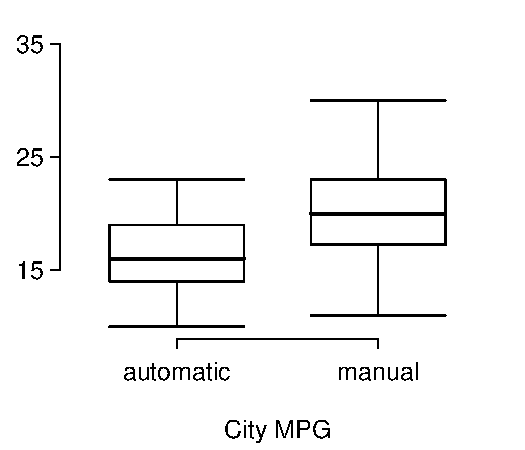
\includegraphics[width=0.6\textwidth]{fuel_eff_city_box.pdf}
\end{center}
\end{minipage}
\end{frame}

\begin{frame}{Example}
\begin{enumerate}[(a)]
\item Write the null and alternative hypothesis for a two sided test.\\
\vspace{1cm}
\item Check the conditions for the test.\\
\vspace{3cm}
\item Calculate the test statistic.\\
\vspace{2.75cm}
\end{enumerate}
\end{frame}

\begin{frame}{Example}
\begin{enumerate}[(a)]
\setcounter{enumi}{3}
\item Calculate the $p$-value and make a decision using $\alpha = 0.01$ significance level.\\
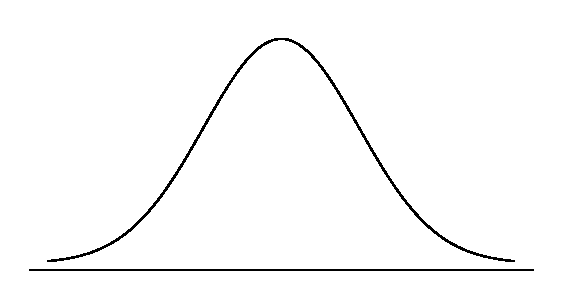
\includegraphics[scale=0.35]{norm_draw.pdf}
\vspace{0.75cm}
\item What is the conclusion of the test in the context of the data?
\vspace{3.5cm}
\end{enumerate}
\end{frame}

\begin{frame}{Example}
\vspace{-4.75cm}
Calculate and interpret a 99\% confidence interval for the difference between the two means.
\end{frame}

%---------------------------------------------
\begin{frame}{Inference for Paired Data}
\begin{itemize}
\item Two sets of observations are \textbf{paired} if each observation in one data set has a correspondence or connection with exactly one observation in the other data set.
\vspace{10pt}
\item To analyze paired data, it is often useful to look at the difference in outcomes of each pair of observations.
\vspace{10pt}
\item Paired data commonly arise in experiments that compare the difference in a variable before and after some treatment was applied to the same subjects (e.g., blood pressure before and after taking a drug).
\end{itemize}
\end{frame}

%---------------------------------------------
\begin{frame}{Inference for Paired Data}
\begin{tabular}{llll}
Case & $x_i$ & $y_i$ & $d_i$\\
\hline
1 & $x_1$ & $y_1$ & $d_1 = x_1 - y_1$\\
2 & $x_2$ & $y_2$ & $d_2 = x_2 - y_2$\\
$\vdots$ & $\vdots$ & $\vdots$ & $\vdots$\\
n & $x_n$ & $y_n$ & $d_n = x_n - y_n$\\
\end{tabular}
\bigskip

Compute the sample mean and standard deviation of the differences:
\begin{align*}
\bar{d} &= \frac{\sum_{i=1}^n d_i}{n}\\
s_d &= \sqrt{\frac{1}{n-1} \sum_{i=1}^n (d_i - \bar{d})^2}\\
\end{align*}
\end{frame}

%---------------------------------------------
\begin{frame}{Inference for Paired Data}
$1-\alpha$ confidence interval for $\mu_d$:
\begin{align*}
\bar{d} \pm t_{\alpha / 2; n-1} \frac{s_d}{\sqrt{n}}\\
\end{align*}

Hypothesis test (paired t-test):\\
$H_0: \mu_d = d_0$\\
$H_A: \mu_d > d_0$, or $\mu_d < d_0$, or $\mu_d \neq d_0$\\
\bigskip

Test Statistic:
\begin{align*}
t = \frac{\bar{d} - d_0}{\frac{s_d}{\sqrt{n}}} \text{; } df=n-1
\end{align*}

Setting $d_0=0$ tests whether the mean difference is 0 (no difference).
\end{frame}

%---------------------------------------------
\begin{frame}{Inference for Paired Data}
Checking the Conditions:\\
\begin{itemize}
\item The paired t-test is just a one-sample t-test applied to the differences.
\vspace{5pt}
\item Check that the sample size is large ($n \geq 30$), or for small samples, that the differences are approximately normal. 
\vspace{5pt}
\item The subjects, or pairs of observations, should be randomly sampled.
\end{itemize}
\end{frame}

%---------------------------------------------
\begin{frame}{Example}
A random sample of $n=170$ British couples were interviewed.  The ages of each husband and wife were recorded, and the first several entries of the data are shown below.  The sample mean difference (husband's age -- wife's age) is $\bar{d} = 2.24$ with standard deviation $s_d = 4.08$.  Use a hypothesis test to determine whether there is a significant difference in age between British husbands and wives.\\
\bigskip

\begin{tabular}{rrrr}
\hline
Case & Husband's Age & Wife's Age & Difference \\
\hline
1 &  49 &  43 &   6 \\
2 &  25 &  28 &  -3 \\
3 &  40 &  30 &  10 \\
4 &  52 &  57 &  -5 \\
5 &  58 &  52 &   6 \\
$\vdots$ & $\vdots$ & $\vdots$ & $\vdots$\\
169 &  40 &  39 &   1 \\ 
170 &  59 &  56 &   3 \\ 
\hline
\end{tabular}
\end{frame}

\begin{frame}{Example}
\begin{enumerate}[(a)]
\item Write the null and alternative hypothesis for a two sided test.\\
\vspace{1cm}
\item Check the conditions for the test.\\
\vspace{3cm}
\item Calculate the test statistic.\\
\vspace{2.75cm}
\end{enumerate}
\end{frame}

\begin{frame}{Example}
\begin{enumerate}[(a)]
\setcounter{enumi}{3}
\item Calculate the $p$-value and make a decision using $\alpha = 0.05$ significance level.\\
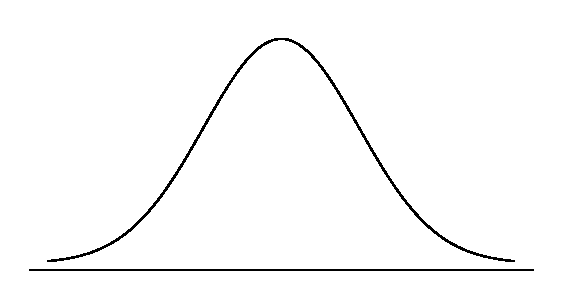
\includegraphics[scale=0.35]{norm_draw.pdf}
\vspace{0.75cm}
\item What is the conclusion of the test in the context of the data?
\vspace{3.5cm}
\end{enumerate}
\end{frame}

\begin{frame}{Example}
\vspace{-4.75cm}
Construct and interpret a 95\% confidence interval for the population mean difference in age between British husbands and wives.
\end{frame}

\end{document}